\documentclass[a4paper, oneside]{article}
\usepackage[utf8]{inputenc}
\usepackage[ngerman]{babel}
\usepackage[top=2.5cm, bottom=3cm, outer=2.5cm, inner=2.5cm, heightrounded]{geometry}
\usepackage{graphicx}
\usepackage{morefloats}
\usepackage{wrapfig}
\usepackage{hyperref}
\usepackage{cite}
\usepackage{siunitx}
\usepackage[default]{sourcesanspro}
\usepackage[T1]{fontenc}
\usepackage{url}
\usepackage{marginnote}
\usepackage[font=footnotesize]{caption}
\usepackage{color}
\usepackage{xcolor}
\usepackage{multicol}
\usepackage[fleqn]{mathtools}
\usepackage{amssymb}
\usepackage{wrapfig}
\usepackage[noindentafter]{titlesec}
\usepackage{fancyhdr}
\usepackage{lastpage}
\usepackage{comment}

%% LÖSUNGEN ANZEIGEN
\newif\ifshow
%\showtrue
\showfalse

%%%SECTIONING
\renewcommand*{\marginfont}{\noindent\rule{0pt}{0.7\baselineskip}\footnotesize}

\newcommand{\aufgabe}[1]{\subsection{#1}}
\newcommand{\loesung}[1]{\subsubsection{#1}}

\newcommand{\simpleset}[1]{\ensuremath \left\{ #1 \right\}}
\newcommand{\ematrix}[2]{\renewcommand{\arraystretch}{1}\ensuremath\left(\begin{array}{@{}#1@{}}#2\end{array}\right)}

\renewcommand{\theenumi}{\alph{enumi})}
\renewcommand{\labelenumi}{\text{\theenumi}}

\newcounter{aufgabe}
%\newenvironment{lsg}{\loesung}{}
\ifshow
  \newenvironment{lsg}{\loesung}{}
\else
  \excludecomment{lsg}
\fi

\newenvironment{inhalt}
  {\paragraph{Inhalt des Übungsblatts:}\itemize\let\origitem\item}
  {\enditemize\vspace{2em}}

\newcommand{\R}{\ensuremath\mathbb{R}}
\newcommand{\N}{\ensuremath\mathbb{N}}
\newcommand{\Z}{\ensuremath\mathbb{Z}}
\newcommand{\LM}{\ensuremath\mathbb{L}}
\newcommand{\intd}{\ensuremath\mathrm{d}}
\newcommand{\e}{\ensuremath\mathrm{e}}
\renewcommand{\d}{\,\mathrm{d}}
\newcommand{\stf}[1]{\ensuremath \left[ #1 \right]}

\newcommand{\cas}{\hfill (CAS)}
\newcommand{\seite}[1]{\textit{(S. #1)}}

\newcommand{\vektor}[1]{\ensuremath\begin{pmatrix} #1 \end{pmatrix}}


\everymath{\displaystyle}

%Malpunkte
\mathcode`\*="8000
{\catcode`\*\active\gdef*{\cdot}}

%SECTION
\titleformat{\section}
{\clearpage\setcounter{aufgabe}{0}\vspace{1em}\Large\raggedright\bfseries}
{}
{0pt}
{}

\titleformat{\subsection}[runin]
{\stepcounter{aufgabe}\vspace{1px}\normalfont\raggedright\bfseries}
{A\theaufgabe: }
{0pt}
{\ }

\titleformat{\subsubsection}[runin]
{\normalfont\raggedright\bfseries}
{Lösung \theaufgabe: }
{0pt}
{\ }


%FANCYHDR
\pagestyle{fancy}
\lhead{\small Simon König\\ Joshua Fabian}
\rhead{\small Mathecrashkurs 2018}
\cfoot{Seite \thepage\thinspace von\thinspace\pageref{LastPage}}
\lfoot{}
\renewcommand{\headrulewidth}{0.5pt}
\renewcommand{\footrulewidth}{0pt}

\title{Mathe-Crashkurs 2018 - Übungsblatt}
\date{\today}
\author{Simon König, Joshua Fabian}

\usepackage{tabularx}

\chead{\Large Probeabitur}
\newcommand{\pts}[1]{\hfill \mbox{(#1 VP)}}
\begin{document}

\section{Pflichtteil}
\aufgabe{} Bilden Sie die erste Ableitung der Funktion $f$ mit $f(x) = (2x^2+5)e^{-2x}$ \pts{2}
\begin{lsg}{}
Es handelt sich um ein Produkt, Anwenden der Produktregel:\\
$u(x) = 2x^2+5 \quad u'(x)=4x$\\
$v(x) = e^{-2x} \quad v'(x)=(-2)e^{-2x}$\\
$\Rightarrow f'(x)=u'(x)v(x)+u(x)v'(x) = 4x\cdot e^{-2x}+(2x^2+5)\cdot(-2e^{-2x})$
\end{lsg}

\aufgabe{} Berechnen Sie das Integral \pts{2}\\
$\int\limits_0^1(2x-1)^4 \intd x$
\begin{lsg}{}
Es handelt sich um eine Verkettung.
Die äußere Funktion ist $x^4$, die innere Funktion ist $2x-1$.\\
\begin{itemize}
  \item  Berechnung der Stammfunktion:
  \begin{align*}
    F(x) &= \frac 1 5 \cdot(2x-1)^5\cdot\frac 1 2\\
    &=\frac{1}{10}\cdot(2x-1)^5
  \end{align*}
  \item Integralberechnung:
  \begin{align*}
    &\int\limits_0^1(2x-1)^4 \intd x\\
    =&\left[\frac{1}{10}\cdot(2x-1)^5\right]^1_0 = \frac{1}{10}-\left(-\frac{1}{10}\right) = \frac 1 5
  \end{align*}
\end{itemize}
\end{lsg}

\aufgabe{}Lösen Sie die Gleichung $\e^x-\frac{3}{\e^x}+2=0$ \pts{3}\\
\begin{lsg}{}
\begin{alignat*}{2}
    &&\e^x-\frac{3}{\e^x}+2 &= 0\\
    \Leftrightarrow\quad && \e^{2x}-3+2\e^x &= 0\\
    \Leftrightarrow\quad && \e^{2x}+2\e^x-3 &= 0\\
    \Leftrightarrow\quad && u^2+2u-3 &= 0 \quad\text{Substitution: }\e^x=u\\
    \Rightarrow\quad && u_{1,2} &= -1\pm\sqrt{1+3}=-1\pm\sqrt{4}=-1\pm2\\
    && u_1 &= -3 \rightarrow \e^x = -3 \quad\text{keine Lösung}\\
    && u_2 &= 1 \rightarrow \e^x = 1 \Leftrightarrow x=0\\
    \LM = \{0\}
\end{alignat*}
\end{lsg}

\aufgabe{}
\begin{multicols}{2}
	Die Abbildung zeigt das Schaubild der Ableitung $f'$ einer Funktion $f$. Skizzieren Sie grob den Verlauf von $f''$ in die Abbildung und geben Sie für jeden der folgenden Sätze an ob er richtig, falsch oder unentscheidbar ist:
	\begin{enumerate}
		\item $f$ schneidet die $y$-Achse bei $(0|1)$.
		\item Das Schaubild von $f$ hat bei $x=-1$ einen Tiefpunkt.
		\item Das Schaubild von $f$ hat für $-2\leq x \leq 2$ genau einen Wendepunkt.
		\item Das Schaubild von $f$ verläuft an der Stelle $1$ steiler als die erste Winkelhalbierede.
		\item $f$ ist im Intervall $[-2;1]$ streng monoton wachsend.
		\item Es gilt $f(3)<f(1)$
		\item $f''$ schneidet die $x$-Achse im Intervall $[1;3]$ zwei mal.
	\end{enumerate}
	\columnbreak
	\centering
	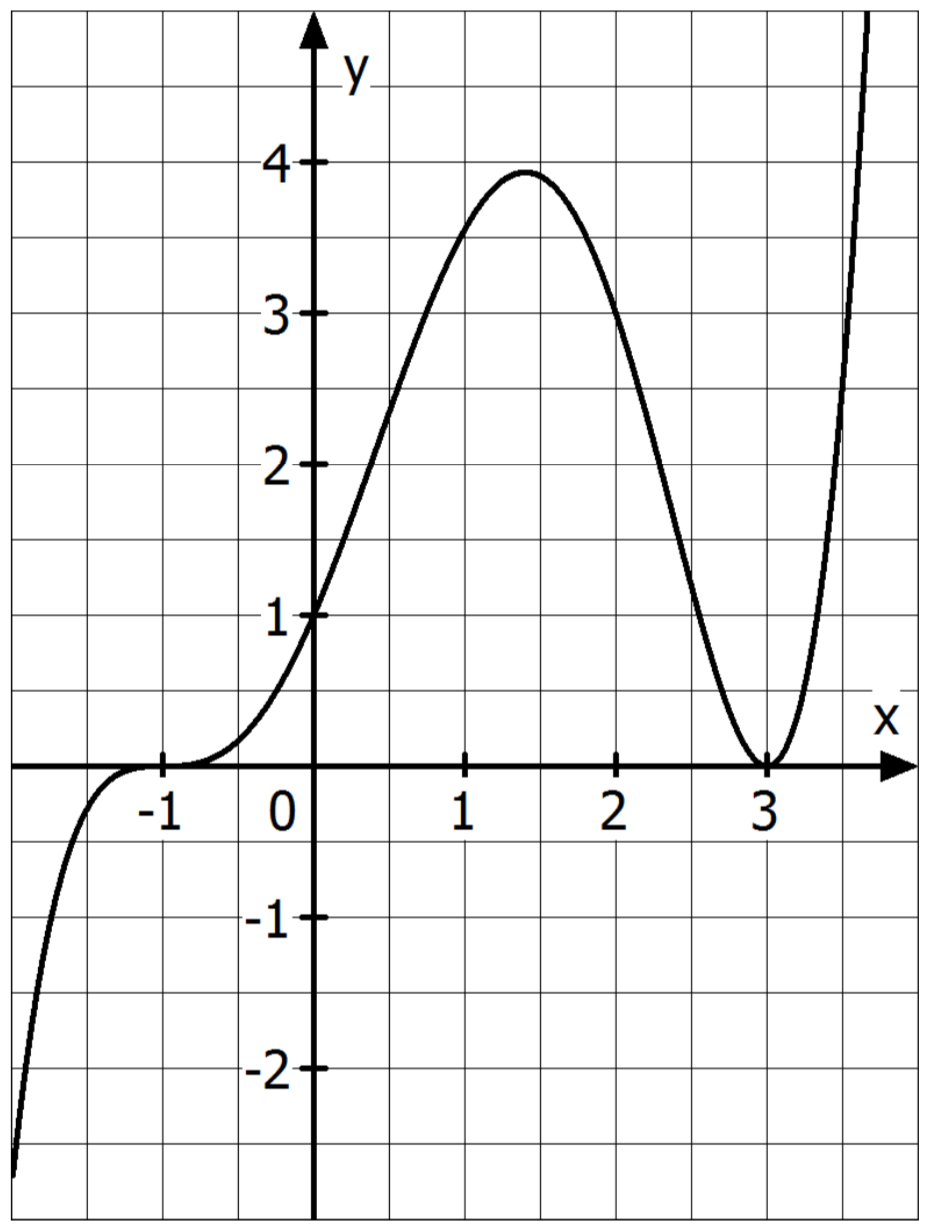
\includegraphics[width=0.7\linewidth]{Monotonieanalyse.png}

	\pts{4}
\end{multicols}
\begin{lsg}{}
	\begin{multicols}{4}
		\begin{enumerate}
			\item unentscheidbar
			\item falsch
			\item richtig
			\item richtig
			\item falsch
			\item falsch
			\item richtig
		\end{enumerate}
	\end{multicols}
\end{lsg}

\aufgabe{}
Gegeben sei die Gerade $g: \vec x=\left(\begin{array}{c} 3 \\ -3 \\ 1 \end{array}\right) + t\cdot \left( \begin{array}{c} 1 \\ 2 \\ 0 \end{array} \right)$ und die Ebene $E = 2x_1-x_2+2x_3=2$. \pts{4}
\begin{enumerate}
  \item Zeigen Sie, dass $E$ und $g$ parallel sind, und berechnen Sie den Abstand von $g$ und $E$.
  \item Die Ebene $F$ ist orthogonal zu $E$ und enthält die Gerade $g$. Bestimmen Sie eine Gleichung der Schnittgeraden von $E$ und $F$.
\end{enumerate}
\begin{lsg}{}
\begin{enumerate}
  \item Für den Normalenvektor der Ebene $E$ gilt: $\vec n_E=\left(\begin{array}{c} 2\\ -1\\ 2\end{array}\right)$. Das Skalarprodukt mit dem Richtungsvektor $\vec u$ von $g$ ist
  \begin{equation*}
    \vec u\bullet\vec n_E = 1\cdot 2 + 2\cdot(-1) + 0\cdot 2 = 0
  \end{equation*}
  d.h. Gerade und Ebene sind parallel.
  \\Der Abstand von $g$ und $E$ ist gleich dem eines beliebigen Punktes von $g$ zu $E$. Wählt man also z.B. den Stützpunkt $P(3|-3|1)$:
  \begin{equation*}
    \mathrm d(g,E)=\mathrm d(P,E)=\frac{|2\cdot3-(-3)+2\cdot1-2|}{3}=\frac{9}{3} = 3.
  \end{equation*}
  \item Da $g$ in $F$ liegt und parallel zu $E$ ist, ist die Schnittgerade $s$ parallel zu g.
  Die Orthogonale $h$ zur Ebene $E$ durch den Stützpunkt $P(3|-3|1)$ von $g$ liegt in $F$ und schneidet $E$ in einem Punkt $S$, den man als Stützpunkt von $s$ wählen kann.
  \begin{equation*}
    \text{Orthognale } h:\vec x = \left(\begin{array}{c}3\\-3\\1\end{array}\right)+t\cdot\left(\begin{array}{c}2\\-1\\2\end{array}\right)
  \end{equation*}
  Schnit von $h$ mit $E$:
  \begin{align*}
    2(3+2t)-(-3-t)+2(1+2t)&=2\\
    9t+11&=2\\
    t&=-1
  \end{align*}
  Einsetzen in die Geradengleichung von $h$ ergibt den Schnittpunkt $S(1|-2|-1)$. Da $g$ und $s$ parallel sind, erhält man mit dem Richtungsvektor von $g$ und $S$ eine Gleichung für die Schnittgerade:
  \begin{equation*}
    s:\vec x=\left(\begin{array}{c}1\\-2\\-1\end{array}\right)+r\cdot\left(\begin{array}{c}1\\2\\0\end{array}\right)
  \end{equation*}
\end{enumerate}
\end{lsg}

\aufgabe{Analytische Geometrie} (vgl. Abitur 2007)\\
Von einem Senkrechten Kegel kennt man die Koordinaten der Spitze $S$, die Koordinaten eines Punktes $P$ des Grundkreises sowie eine Koordinatengleichung der Ebene $E$, in der der Grundkreis liegt.
\\Beschreiben Sie ein Verfahren, um den Mittelpunkt $M$ und den Radius $r$ des Grundkreises zu bestimmen.

\pts{3}
\begin{lsg}{}
\begin{itemize}
  \item Mit der Koordinatengleichung $ax_1+bx_2+cx_3=d$ ist der Normalenvektor $\vec n_E=\left(\begin{array}{c}a\\b\\c\end{array}\right)$ von $E$ gegeben.
  Das Lot $l$ von $S$ auf $E$ hat $\vec n_E$ als Richtungsvektor.
  \item Der Durchstoßpunkt von $l$ durch $E$ ist der Mittelpunkt $M$ des Grundkreises.
  \item Der Betrag des Vektors $\overrightarrow{MP}$ ist der Radius $r$ des Grundkreises.
\end{itemize}
\end{lsg}

\aufgabe{Stochastik} (vgl. Abitur 2017)\\
In einer Urne liegen drei rote, zwei grüne und eine blaue Kugel. Es werden so lange nacheinander einzelne Kugeln gezogen und zur Seite gelegt, bis man eine rote Kugel erhält. Bestimmen Sie die Wahrscheinlichkeit dafür, dass man höchstens drei Kugeln zieht. \pts{2}
\begin{lsg}{}
3 Rot, 2 Grün, 1 Blau. Insgesamt 6.

$\frac 3 6 + \frac 3 6 \cdot\frac 3 5 + \frac 3 6 \cdot \frac 2 5 \cdot \frac 3 4 = \frac 1 2+\frac{9}{30} +\frac{18}{120}=\frac 1 2 + \frac{3}{10}+  \frac{3}{20} = \frac{19}{20}$
\end{lsg}

\vfill

\hfill\rule{1.5cm}{0.4mm}

\hfill (20 VP)\hspace{0.22cm}







\section{Wahlteil Analysis}

\aufgabe{} (vgl. Abitur 2006)\\
Gegeben ist die Funktion von f durch:
\begin{equation*}
  f(x)=\frac{120(x-120)^2}{(x-120)^2+7200} + 10 \quad\text{mit $0\leq x \leq 130$}
\end{equation*}
Ihr Schaubild sei K. Das Schaubild der Funktion g mit $g(x)=-0.015x^2+0.15x+95$ sei C.

Eine Skisprunganlage besteht aus Sprungschanze und Aufsprunghang. Das Schaubild K beschreibt das Profil des Aufsprunghangs, die Kurve C die Flugbahn eines Skisprungers. Der Absprung erfolgt bei $x=0$. Alle Angaben in Metern.

\begin{enumerate}
  \item Bestimmen Sie die Koordinaten des Punktes, an dem der Springer auf dem Aufsprunghang aufsetzt. Wie groß ist die maximale vertikal gemessene Höhe des Springers über dem Hang? \pts{2}
  \item Der Wendepunkt $W(71|40)$ von K entspricht dem kritischen Punkt des Aufsprunghangs. Mögliche Flugbahnen des Skispringers werden nun durch Schaubider der Funktionen $g_k=-0.015x^2+kx+95$ beschrieben. Welchen Wert darf der Parameter k höchstens annehmen, damit der Springer mit dieser Flugbahn nicht hinter dem kritrischen Punkt landet? \pts{3}
  \item Beim Umbau dieser Schanze soll das Profil des Aufsprunghangs verändert werden. Er soll nach dem Umbau durch die Funktion h mit
  \begin{equation*}
    h(x)=0.0001(1,25x^3-225x^2+2150x+900000) \quad\text{mit $0\leq x \leq 130$}
  \end{equation*}
  beschrieben werden. Muss zur Realisierung des neuen Profils insgesamt Erde weggefahren oder angeliefert werden, wenn angenommen wird, dass der Hang überall gleich breit ist? \pts{3}
\end{enumerate}
\begin{lsg}{}
\begin{enumerate}
	\item Gleichsetzen der Funktionen $f$ und $g$ mit $0\leq x \leq 130$ ergibt $S(60|50)$ als Schnittpunkt.

	Für die maximale vertikale Höhe wird die Differenzfunktion aufgestellt: $d(x)\coloneqq g(x)-f(x)$. Nun ist der Hochpunkt von $d$ gesucht. Dieser befindet sich bei $x_{max}\approx26,08$. $d(x_{max})=12,64$.
	\item $g_k$ muss $f$ spätestens im Punkt $W(71|40)$ schneiden, berechnen des $k$, sodass sich $g_k$ und $f$ in $W$ schneiden:
	\begin{equation*}
		g_k(71)=f(71) \rightsquigarrow k\leq 0,29
	\end{equation*}
	\item Berechnung der Integrale der beiden Funktionen $f$ und $h$ im Intervall $[0;130]$:
	\begin{align*}
		\int\limits_0^{130} f(x)\d x &= 5978,15\\
		\int\limits_0^{130} h(x)\d x &= 5964,56
	\end{align*}
	Das das neue Profil eine geringere Querschnittsfläche besitzt, muss Erde weggefahren werden.
\end{enumerate}
\end{lsg}


\aufgabe{} (vgl. Abitur 2015)
Gegeben sind ein Kreis mit Mittelpunkt $O(0|0)$ und die Funktion f mit $f(x)=\frac{4}{x^2+1}$. Bestimmen Sie die Anzahl der gemeinsamen Punkte des Kreises mit dem Graphen von f in Abhängigkeit vom Kreisradius. \pts{4}

\begin{lsg}{}
Für die Entfernung des Punktes $P(u|f(u))$ vom Ursprung gilt:
$d(u)=\sqrt{u^2+(f(u))^2}$ Gesucht ist das Minimum:
$d_{\mathrm{min}}\approx 1,94$ d.h. der Kreis mit dem Radius $d_{\mathrm{min}}$ berührt den Graphen in genau zwei Punkten.
Der Kreis mit Radius 4 geht durch den Hochpunkt und hat damit 3 Schnittpunkte.

\bigskip
\noindent
\begin{tabular}{c | c}
  Radius & Schnittpunkte\\
  \hline $0<r<d_{\mathrm{min}}$ & 0\\
  $r=d_{\mathrm{min}}$ & 2\\
  $d_{\mathrm{min}}<r<4$ & 4\\
  $r=4$ & 3\\
  $r>4$ & 2
\end{tabular}
\end{lsg}

\aufgabe{}
Für jedes $t\in \R$ ist die Funktion $g_t$ mit
\begin{equation*}
	g_t(x)=\e^{t-x}+x
\end{equation*}
gegeben.
\begin{enumerate}
	\item Der Graph jeder Funktion $g_t$ besitzt einen Tiefpunkt $T_t$. Bestimmen Sie die Ortskurve dieser Tiefpunkte. \pts{3}
	\item Der Graph von $g_0$, die $y$-Achse und die erste Winkelhalbierede begrenzen eine nach rechts offene Fläche mit endlichem Inhalt. Berechnen sie den Inhalt dieser Fläche.

	Die Gerade $x=a$ mit $a>0$ halbiert diese Fläche. Bestimmen Sie den Wert von $a$ exakt. \pts{5}
\end{enumerate}
\begin{lsg}{}
	\begin{enumerate}
		\item Koordinaten der Tiefpunkte: $T_t(t|1+t) \rightsquigarrow$ Gleichung der Ortskurve $y_t(x)=x+1$
		\item $A(z)=\int\limits_0^z(g_0(x)-x)\d x=-\e^{-z}+1$

		Dann ergibt sich für den Grenzwert $A=\lim\limits_{z\rightarrow \infty} (-\e^{-z}+1)=1$

		Halbierung der Fläche, gesucht ist der Wert von $a$ so, dass $A(a)=\frac 1 2$.

		\begin{align*}
			-\e^{-a}+1 &= \frac 1 2\\
			\e^{-a} &= \frac 1 2\\
			-a &= \ln\left(\frac 1 2\right)\\
			-a &= -\ln(2)\\
			a = \ln(2)
		\end{align*}
	\end{enumerate}
\end{lsg}






\vfill

\hfill\rule{1.5cm}{0.4mm}

\hfill (20 VP)\hspace{0.22cm}





\section{Wahlteil Analytische Geometrie}

Gegeben sind die Gerade $g$ durch die Punkte $A(0|-4|1)$ und $B(1|-2|0)$ sowie für jedes $a\in\R$ eine Ebene $E_a$ durch $x_1+(a-1)x_2+2ax_3=-2a+1$.
\begin{enumerate}
  \item Berechnen Sie den Schnittpunkt von $g$ mit der Ebene $E_0$.\\
  Begründen Sie, dass $A$ und $B$ auf der gleichen Seite der Ebene $E_0$ liegen.\\
  Bestimmen Sie den Schnittwinkel von $g$ und der Ebene $E_0$. \pts{2,5}

  \item Berechnen Sie den Wert von $a$, für den die Ebene $E_a$ parallel zur $x_2$-Achse ist. Für welche Werte von $a$ mit $-1\leq a\leq 1$ schneidet die $x_1$-Achse die Ebene $E_a$ unter einem Winkel von 45$^\circ$? \pts{3}

  \item Zeigen Sie, dass eine Gerade $h$ gibt, die in allen Ebenen $E_a$ liegt. \pts{2,5}

  \item Welcher Punkt der $x_3$-Achse liegt in keiner Ebene $E_a$? \pts{2}
\end{enumerate}
\begin{lsg}{}
	\begin{enumerate}
		\item $S(3|2|-2)$

		Wegen $\vec{OS}=\vec{OA}+3\vec{AB}$ liegt $S$ nicht zwischen $A$ und $B$.

		$\alpha = 16,8^\circ$

		\item $E_a || x_2$-Achse, wenn $\vec{n_{E_a}}*\vec{u_a}=0 \rightsquigarrow a=1$ Ebene $E_a$ ist parallel zur $x_2$-Achse

		Es muss gelten: $\sin(45^\circ)=\frac{|u_1*n_a|}{|u_1|*|n_a|} \rightsquigarrow a_1=0, a_2=0,4$

		\item Schnittgerade von $E_0$ und $E_1$ berechnen und zeigen, dass sie in allen Ebenen $E_a$ liegt.

		\begin{equation*}
			h: \vec x=\vektor{-1\\-2\\0}+t*\vektor{-2\\-2\\1}
		\end{equation*}

		\item $P(0|0|s)$ in $E_a$ einsetzen $\rightsquigarrow a=\frac{1}{2(s+1)} \rightsquigarrow s\not=-1$

		$P(0|0|-1)$ liegt in keiner Ebene $E_a$
	\end{enumerate}
\end{lsg}



\vfill

\hfill\rule{1.5cm}{0.4mm}

\hfill (10 VP)\hspace{0.22cm}


\section{Wahlteil Stochastik}
Die Tabelle zeigt die Häuftigkeitsverteilung von Rauchern und Nichtrauchern unter den Personen im Alter von 50 bis 55 Jahren in Deutschland.

\vspace{2em}
\begin{tabular}{ c|c }
	Raucher & Nichtraucher\\
	gelegentlich: 4,0\%, regelmäßig: 28,1\% & früher geraucht: 22,1\%,  nie geraucht: 45,8\%
\end{tabular}
\vspace{2em}

\noindent
Im Folgenden werden nur Personen der angegebenn Altersgruppe betrachtet.
\begin{enumerate}
	\item Zwanzig zufällig ausgewählte Personen gehen nacheinander zu einer Gesundheitsuntersuchung. Bestimmen Sie die Wahrscheinlichkeiten der folgenden Ereignisse:
	\begin{itemize}
		\item A: Genau acht Personen sind Raucher.
		\item B: Mehr als acht Personen haben noch nie geraucht.
		\item C: Genau acht Personen sind Raucher, wobei die letze Person ein Raucher ist.
		\item D: Die ersten drei Personen sind Nichtraucher und von den übrigen rauchen mindestens sechs regelmäßig.
	\end{itemize}
	\item Acht Raucher beginnen ihre Entwöhnungskur. Sieben von ihnen sind regelmäßige Raucher. Die Erfolgschancen betragen unabhängig voneinander für regelmäßige Raucher 60\%, für Gelegenheitsraucher 80\%. Berechnen Sie die Wahrscheinlichkeit dafür, dass mindestens sieben Personen die Kur mit Erfolg beenden.
	\item Eine Krankenkasse gewährt ihren Mitgliedern einen Bonus, wenn sie Nichtraucher sind. Wie groß müsste der Anteil der Nichtraucher unter ihren Mitgliedern im Alter von 50-55 Jahren mindestens sein, damit von 100 zufällig ausgewählten Mitgliedern dieser Altersgruppe mit einer Wahrscheinlichkeit von mindestens 90\% mindestens 70 den Bonus erhalten.
\end{enumerate}


\begin{lsg}{}
	\newcommand{\bin}[1]{\ensuremath\mathrm{B}_{#1} \text{-verteilt}}
	\begin{enumerate}
		\item
		\begin{itemize}
			\item $X_1$ beschreibt die Anzahl der Raucher unter 20 Personen. $X_1$ kann als $\bin{20;0,321}$ angenommen werden.

			$P(A)=P(X_1=8)=0,1364\approx 13,6\%$
			\item $X_2$ beschreibt die Anzahl der Personen, die noch nie geraucht haben, unter 20 Personen an.

			$X_2$ kann als $\bin{20;0,458}$ angenommen werden.

			$P(B)=P(X_1>8)=0,6137\approx 61,4\%$
			\item Der letzte ist Raucher, d.h. vorher 7 Raucher. $X_3$ beschreibt die Anzahl der Raucher unter 19 Personen.

			$X_3$ kann als $\bin{19;0,321}$ angenommen werden.

			$P(C)=P(X_1=7)*0321=0,0546\approx 5,5\%$
			\item Die ersten drei Nichtraucher $X_4$ beschreibt die Anzahl der regelmäßigen Raucher unter 17 Personen.

			$X_2$ kann als $\bin{20;0,458}$ angenommen werden.

			$P(B)=0,679^3*P(X_1\geq6)=0,1053\approx 10,5\%$
		\end{itemize}
		\item Es gibt zwei Pfade: 6 regelmäßige Raucher und ein Gelegenheitsraucher bestehen die Kur oder 7 regelmäßige Raucher schaffen es.

		$w=P(X=7)*0,8+P(X=7)*0,2+P(X=6)*0,8=0,1325\approx 13,3\%$
		\item Der Anteil der Nichtraucher unter unter den Mitgliedern der Krankenkasse sei p.

		$Y$ beschreibt die Anzahl der Nichtraucher unter 100 Mitgliedern. $Y$ kann als $\bin{100;p}$ gesehen werden.

		Gesucht ist die kleinste positive Zahl $p$ mit $P(Y\geq 70)\geq 0,9$

		Mit dem Tabellenmodus des CAS erhält man $p=0,751: P(Y\geq 70\approx 0,9004$ und $p=0,750: P(Y\geq 70\approx 0,8962$. Somit ist $p=0,751$ der gesuchte Wert.

		Somit müsste der Nichtraucheranteil mindestens $75,1\%$ betragen.
	\end{enumerate}
\end{lsg}

\vfill

\hfill\rule{1.5cm}{0.4mm}

\hfill (10 VP)\hspace{0.22cm}

\end{document}
